\newpage
\section{Работа поликлиники}

\subsection{Создание расписания работы врачей}

Расписание работы врачей, ведущих амбулаторный прием, должно регулярно создаваться на последующий период работы ЛПУ в случае, если в ЛПУ организован прием пациентов по предварительной записи или по талонам. В зависимости от организации работы в конкретном ЛПУ, период, на который составляется расписание может быть различным. Рекомендуется создавать расписание на календарный месяц. Однако, возможно создание расписания и на более короткий (или более продолжительный) период.

Для доступа к созданию и редактированию расписания приема врачей необходимо нажать кнопку \btn{Формирование графика врача} вверху страницы на панели управления, либо нажать на блок \dm{Графики работы врачей} на главной странице системы (Рисунок \ref{img_gen_main}). Будет осуществлен переход на страницу \dm{График врача} (Рисунок \ref{img_pol_ttbl1}).

\begin{figure}[ht]\centering
 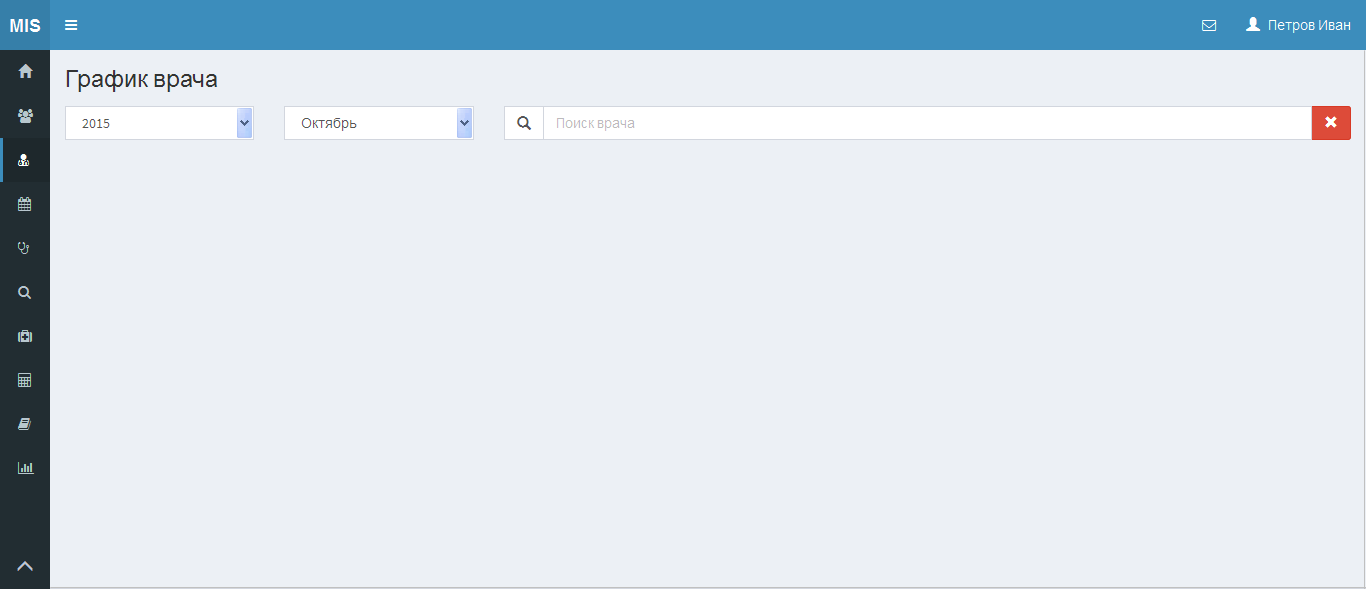
\includegraphics[width = 1\textwidth ,keepaspectratio]{pol_ttbl1}
 \caption{Страница выбора графика работы}
 \label{img_pol_ttbl1}
\end{figure}

На открывшейся странице необходимо выполнить следующие действия:
\begin{enumerate}
 \item В первом поле выбрать номер года для составления расписания.
 \item Во втором поле выбрать месяц, на который планируется составить расписание.
 \item В третьем поле указать имя сотрудника, для которого планируется составление расписания. По мере ввода текста в данное поле, осуществляется фильтрация списка сотрудников по введенным буквам. Отбираются сотрудника, фамилия или специальность которых начинается с указанных символов. Когда имя искомого сотрудника появится на экране, следует выбрать его из выпадающего списка, щелкнув по нему левой кнопкой мыши. На экране появится расписание выбранного сотрудника за указанный месяц (Рисунок \ref{img_pol_ttbl2}).
 \item Нажать кнопку \btn{Редактировать} в левой части страницы. 
\end{enumerate}

\begin{figure}[ht]\centering
 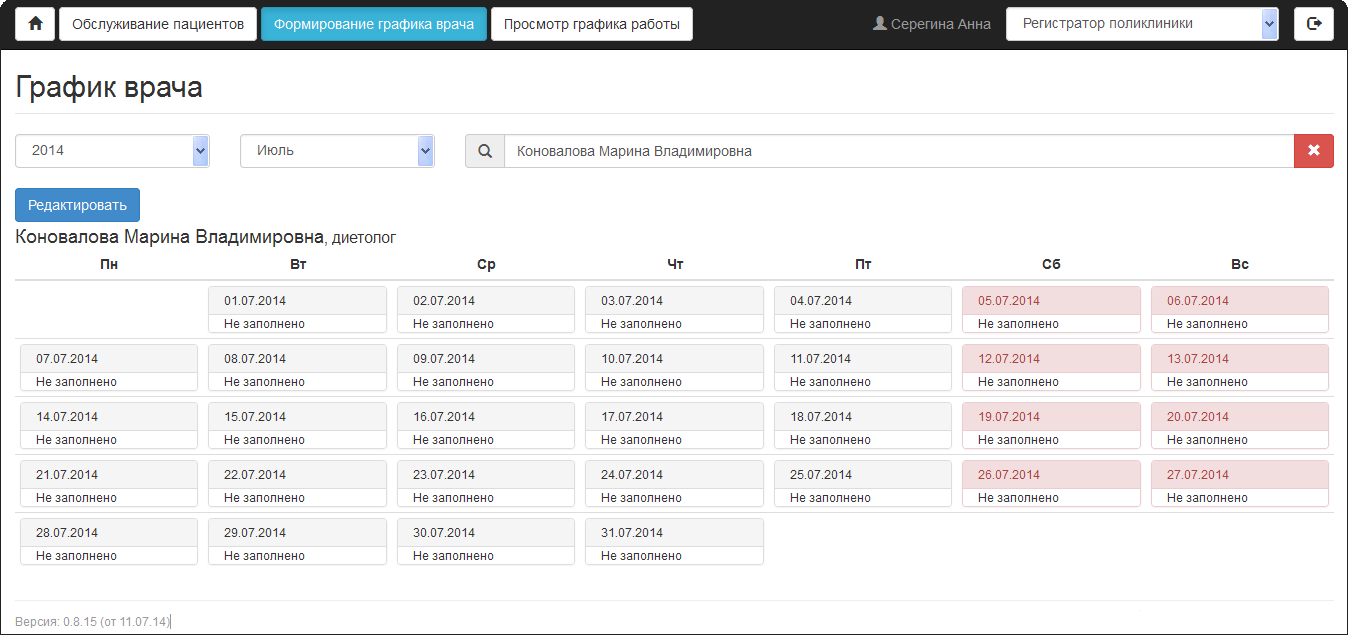
\includegraphics[width = 1\textwidth ,keepaspectratio]{pol_ttbl2}
 \caption{График работы сотрудника}
 \label{img_pol_ttbl2}
\end{figure}

В результате выполнения вышеперечисленных действий расписание станет доступно для редактирования, на экране появятся дополнительные кнопки управления расписанием (Рисунок \ref{img_pol_ttbl3}):
\begin{itemize}
 \item Кнопка \btn{Сохранить} позволяет сохранить созданное расписание сотрудника.
 \item Кнопка \btn{Отменить} осуществляет выход из режима редактирования расписания. Все несохраненные изменения будут потеряны.
 \item Кнопка \btn{Заполнить} позволяет заполнить расписание работы сотрудника на выделенные дни. Кнопка доступна, если выделен хотя бы один день расписания.
 \item Кнопка \btn{Нечет дни} выделяет все нечетные дни месяца. Если флажок \dm{Выбирать выходные} установлен, то выделяются все нечетные дни, включая выходные. В противном случае - только нечетные рабочие дни.
 \item Кнопка \dm{Инверсия} инвертирует выделение дней расписания, т.е. снимает выделение с ранее выделенных дней и выделяет все дни, которые были не выделены. Для того чтобы выделить все четные дни, следует последовательно нажать кнопки \btn{Нечет дни} и \btn{Инверсия}. Если флажок \dm{Выбирать выходные} НЕ установлен, то выходные дни не будут выделяться вне зависимости от того, были ли они выделены до нажатия кнопки \btn{Инверсия}.
 \item Кнопка \btn{Все} позволяет выделить все дни месяца. Если флажок \dm{Выбирать выходные} НЕ установлен, то выделяются все рабочие дни месяца.
 \item Кнопка \btn{Снять} снимает все выделения.
 \item Кнопки 
\includegraphics[scale=0.6]{arr1}, расположенные слева, напротив каждой недели,   позволяют выделить все дни выбранной недели. Если флажок \dm{Выбирать выходные} установлен, то выделяются все дни, в противном случае - только рабочие дни.
\end{itemize}

Можно так же выделять дни в произвольном порядке, щелкая по ним левой кнопкой мыши. Для снятия выделения с дня следует щелкнуть по нему левой кнопкой мыши повторно.

\begin{figure}[ht]\centering
 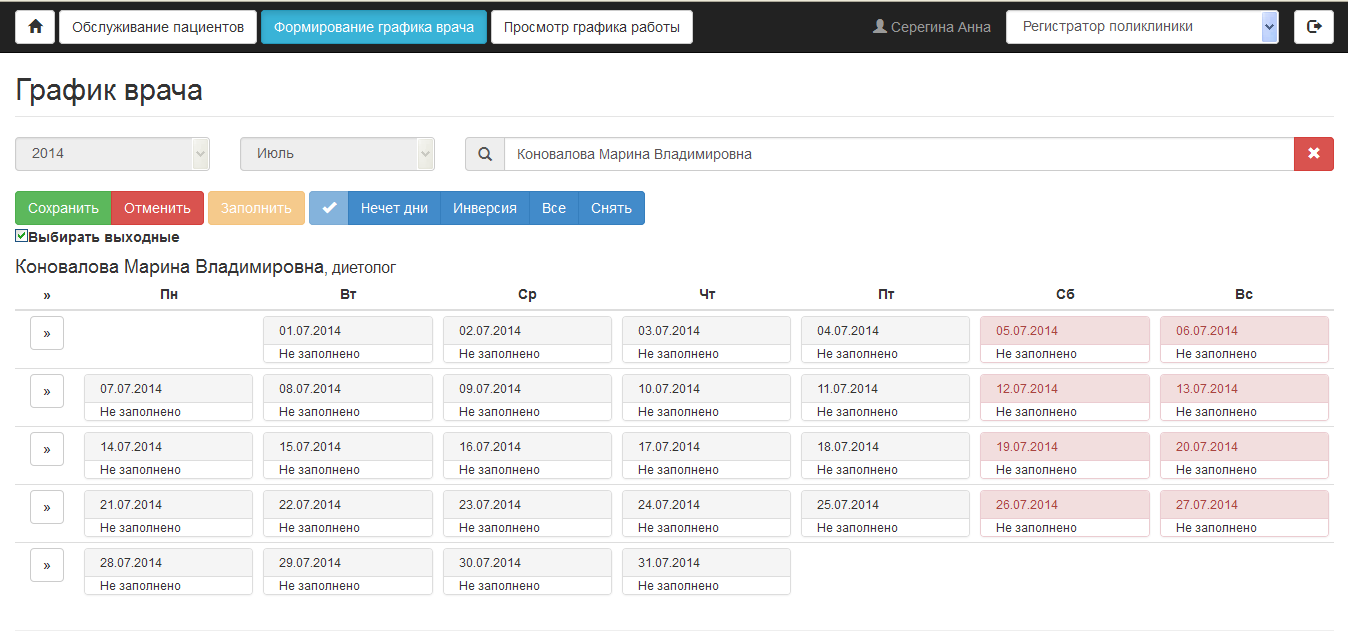
\includegraphics[width = 1\textwidth ,keepaspectratio]{pol_ttbl3}
 \caption{Редактирование расписания сотрудника}
 \label{img_pol_ttbl3}
\end{figure}

Необходимо выделить один или несколько дней, расписание на которые совпадает, любым из описанных способов и нажать кнопку \btn{Заполнить}. Откроется окно \dm{Заполнение расписания} (Рисунок \ref{img_pol_ttbl4}). 

\begin{figure}[ht]\centering
 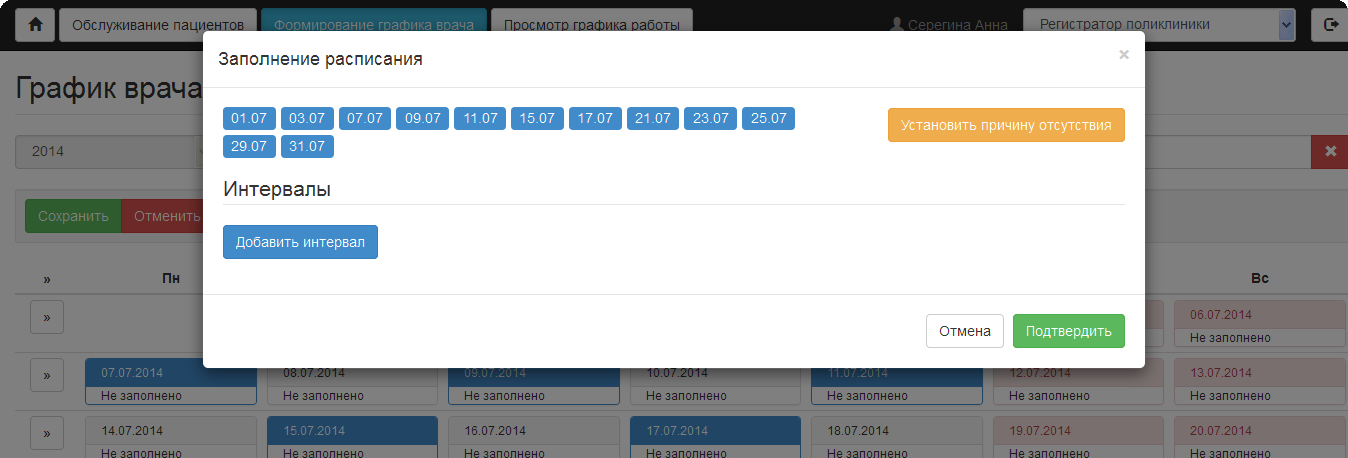
\includegraphics[width = 1\textwidth ,keepaspectratio]{pol_ttbl4}
 \caption{Окно <<Заполнение расписания>>}
 \label{img_pol_ttbl4}
\end{figure}

В открывшемся окне в правом верхнем углу будут перечислены дни, на которые будет сформировано расписание в результате текущей операции. Следует нажать кнопку \btn{Добавить интервал} и заполнить появившиеся поля:
\begin{itemize}
 \item \dm{Тип} -- тип приема выбирается из списка (Амбулаторно или на дому);
 \item \dm{Время начала приема};
 \item \dm{Время конца приема};
 \item \dm{Кабинет} -- кабинет, в котором ведется прием. Поле доступно только, если выбран амбулаторный тип приема.
\end{itemize}
Все перечисленные поля, за исключением последнего, являются обязательными для заполнения.  Поле \dm{Кабинет} является обязательным только для амбулаторного типа приема.

Допускается добавление нескольких интервалов в рамках одного дня приема, в том числе нескольких интервалов одного типа. Для добавления нового интервала необходимо нажать кнопку \btn{Добавить интервал} еще раз и заполнить вновь появившиеся поля.

Для каждого типа приема, запланированного на текущий день, необходимо заполнить плановые показатели по приему пациентов. Для этого в области слева от данных интервала приема следует заполнить поля:
\begin{itemize}
 \item \dm{План приема} -- плановое количество пациентов, которых должен принять врач за день. Соответствует количеству талонов, которые будут созданы на текущий день для выбранного типа приема. Является обязательным для заполнения;
 \item \dm{Сверх плана} -- допустимое количество пациентов, которые могут быть записаны дополнительно (без талонов);
 \item \dm{Вне очереди} -- допустимое количество экстренных пациентов, которые могут приняты данным врачом без талона в течении дня.
\end{itemize}

После заполнения расписания окно будет выглядеть следующим образом (Рисунок \ref{img_pol_ttbl5}). После нажатия кнопки \btn{Подтвердить}, расположенной в правом нижнем углу окна, будет заполнено расписание на выбранные дни в соответствии с заданным шаблоном. Далее следует выделить следующую группу дней с одинаковым графиком работы сотрудника и, вызвав окно заполнения расписания, создать расписание на эти дни. Операцию заполнения следует повторять до тех пор, пока не будет заполнено расписание на все дни периода. В результате, окно формирования графика врача примет следующий вид (Рисунок \ref{img_pol_ttbl6}). Необходимо нажать кнопку \btn{Сохранить} для внесения расписания в БД. 

\begin{figure}[ht]\centering
 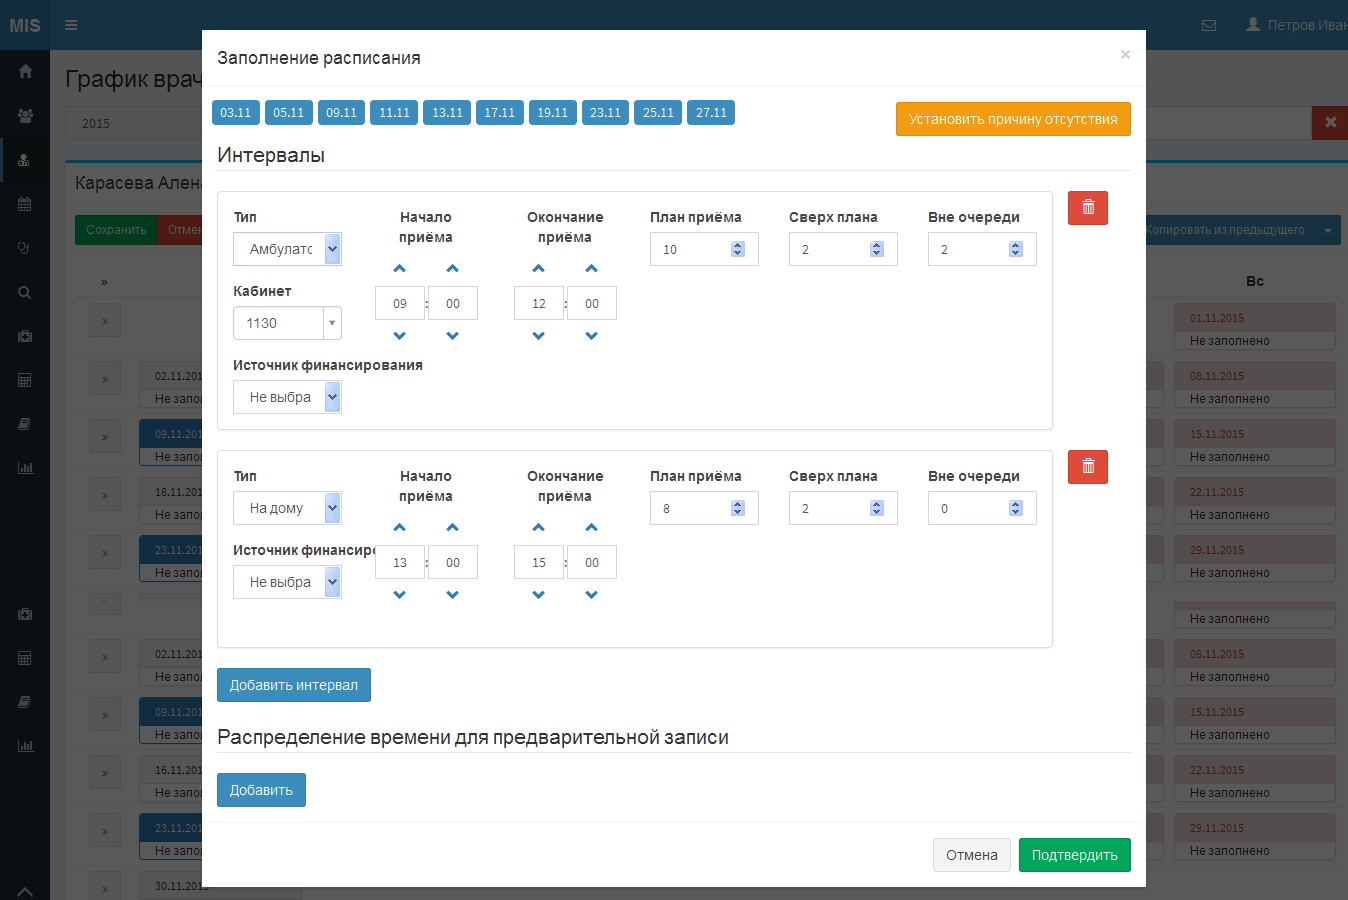
\includegraphics[width = 1\textwidth ,keepaspectratio]{pol_ttbl5}
 \caption{Окно <<Заполнение расписания>> после внесения данных}
 \label{img_pol_ttbl5}
\end{figure}

\begin{figure}[ht]\centering
 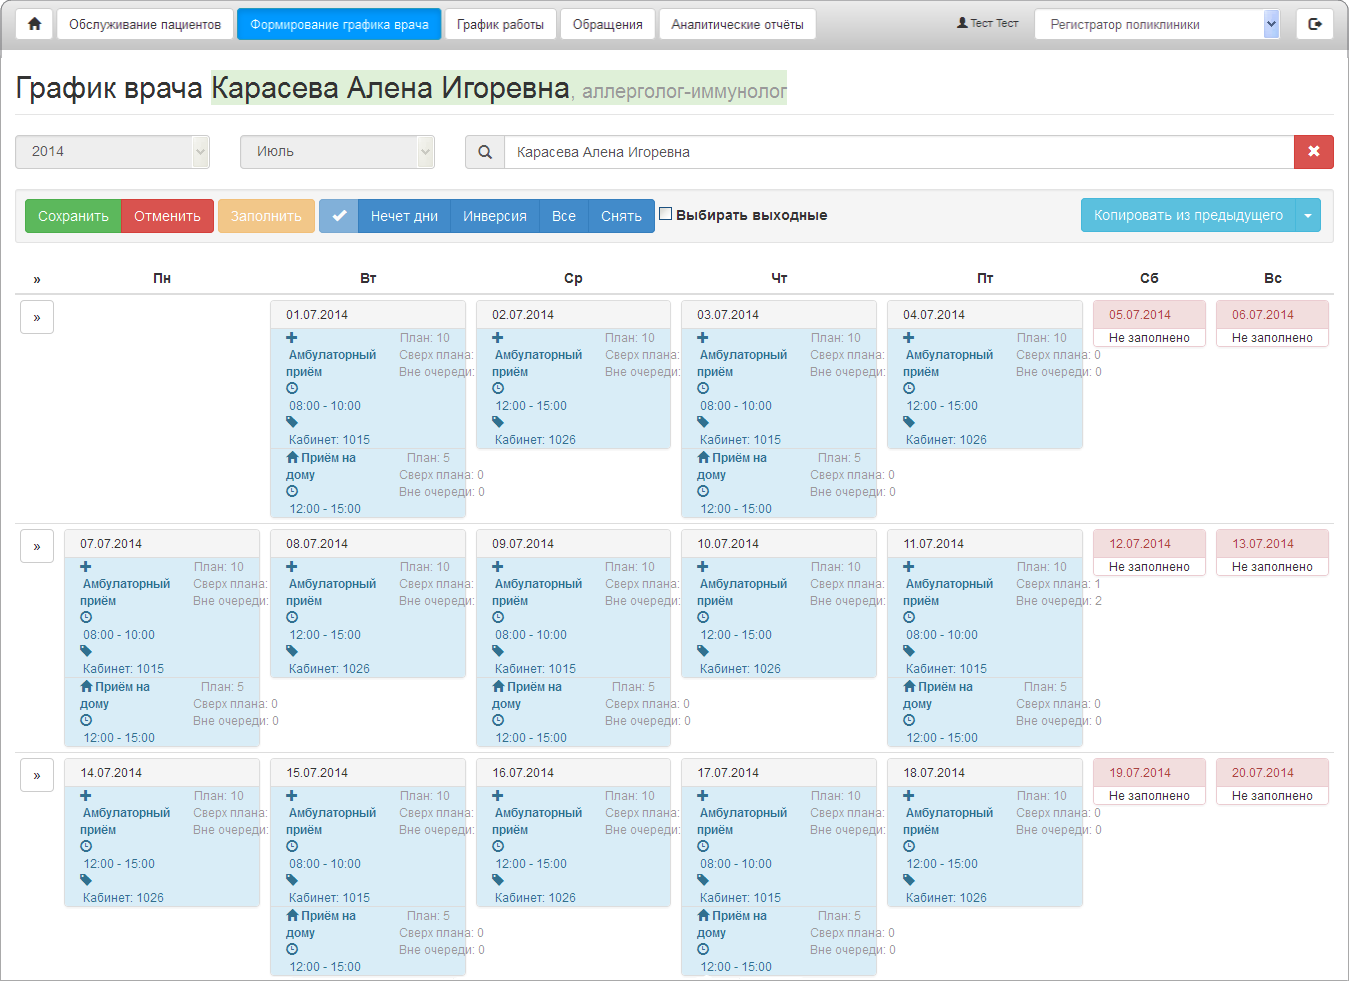
\includegraphics[width = 1\textwidth ,keepaspectratio]{pol_ttbl6}
 \caption{Заполненное расписание сотрудника}
 \label{img_pol_ttbl6}
\end{figure}

\subsubsection{Регистрация отсутствий сотрудников}

Если врач не может вести прием по какой-либо причине, необходимо отметить его отсутствие в расписании. Для этого следует открыть расписание сотрудника на соответствующий период на редактирование, выбрать дни отсутствия и нажать кнопку \btn{Заполнить}. Откроется всплывающее окно \dm{Заполнение расписания}. В левом верхнем углу окна нужно нажать кнопку \btn{Установить причину отсутствия} и в появившемся под кнопкой поле выбрать из списка причину отсутствия. После этого следует нажать кнопку \btn{Подтвердить} в правом нижнем углу окна. Расписание сотрудника на выбранные дни будет удалено, а в полях расписания будет указана выбранная причина отсутствия (Рисунок \ref{img_pol_ttbl7}). После сохранения расписания, оно станет недоступным для записи из регистратуры.

\begin{vnim}
 Не забудьте сохранить расписание после внесения информации об отсутствиях кнопкой \btn{Сохранить}.
\end{vnim} 

\begin{figure}[ht]\centering
 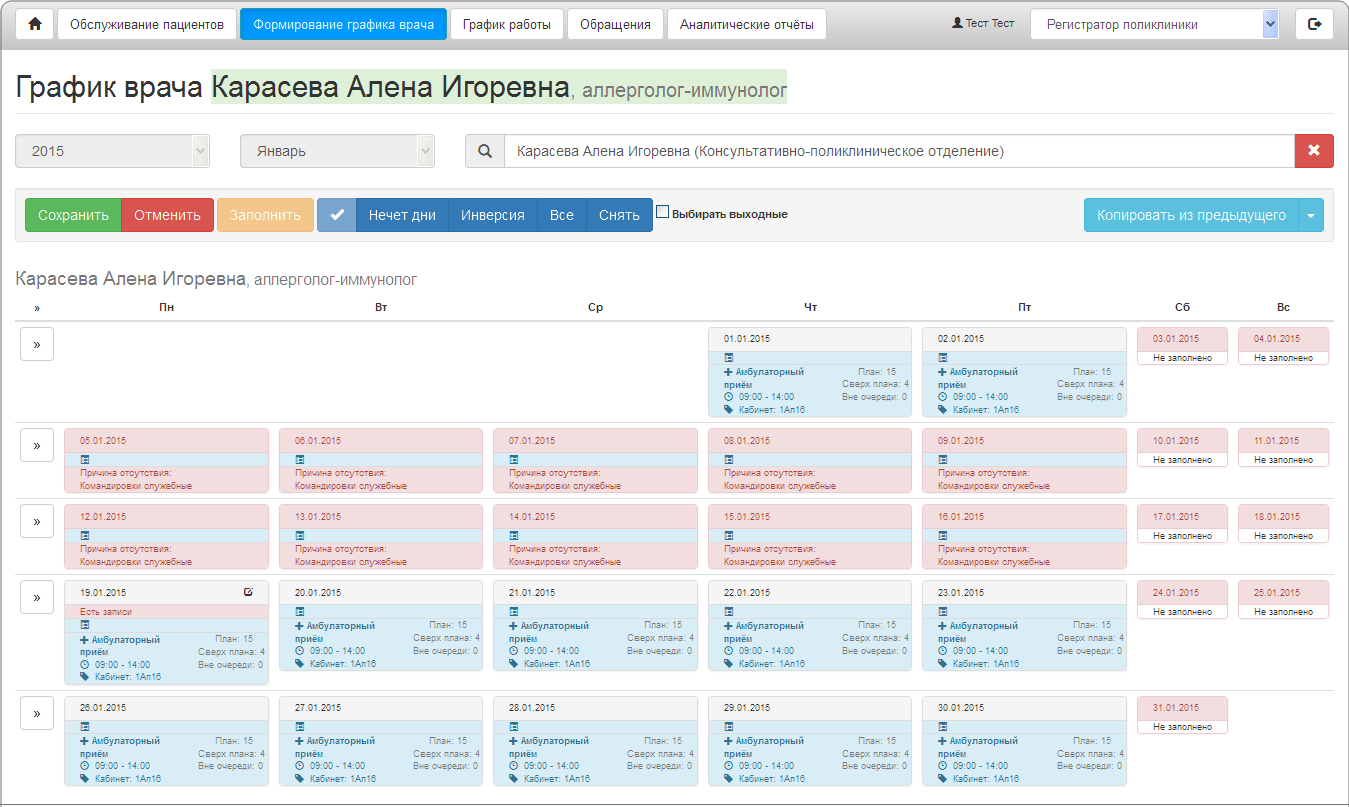
\includegraphics[width = 1\textwidth ,keepaspectratio]{pol_ttbl7}
 \caption{Отсутствия сотрудника}
 \label{img_pol_ttbl7}
\end{figure}

Если необходимо отменить запись об отсутствии сотрудника, следует выделить дни, в которые нужно отменить ранее установленное отсутствие и нажать кнопку \btn{Заполнить}. Появится всплывающее окно \dm{Заполнение расписания}. В левом верхнем углу появившегося окна следует нажать кнопку \btn{Убрать причину отсутствия} и нажать кнопку \btn{Подтвердить} для внесения изменений. Запись об отсутствии сотрудника будет удалена, однако расписание сотрудника на эти дни нужно будет создать заново. 

\subsection{Предварительная запись на прием}

Предварительная запись пациентов на прием осуществляется на странице обслуживания пациентов. Для перехода на эту страницу необходимо нажать кнопку \btn{Обслуживание пациентов} вверху страницы на панели управления, либо нажать на блок \dm{Обслуживание пациентов} на главной странице системы (Рисунок \ref{img_gen_main}).

Последовательность действий при записи пациента на прием должна быть следующая:
\begin{enumerate}
 \item Найти пациента в картотеке (см. раздел \ref{cl_find}) Если пациент не был зарегистрирован ранее, его следует зарегистрировать (см. раздел \ref{cl_new})
 \item Щелкнуть левой кнопкой мыши по записи о пациенте в списке найденных пациентов и в появившемся всплывающем окне (Рисунок \ref{img_cl_contrwin}) нажать кнопку \btn{Записать на прием}. Откроется страница \dm{Запись пациента на прием}. Кнопка \btn{Записать на прием} доступна так же в правом верхнем углу регистрационной карточки пациента.  
 \item В правой части окна, в поле поиска врача, ввести фамилию или специальность врача. В результате, список врачей, расположенный ниже поля поиска, будет отфильтрован согласно условиям поиска.
 \item Установить флажок напротив фамилии нижного врача. На экране появится расписание выбранного сотрудника на текущую неделю (Рисунок \ref{img_pol_zapttbl}).
 
 \begin{figure}[ht]\centering
  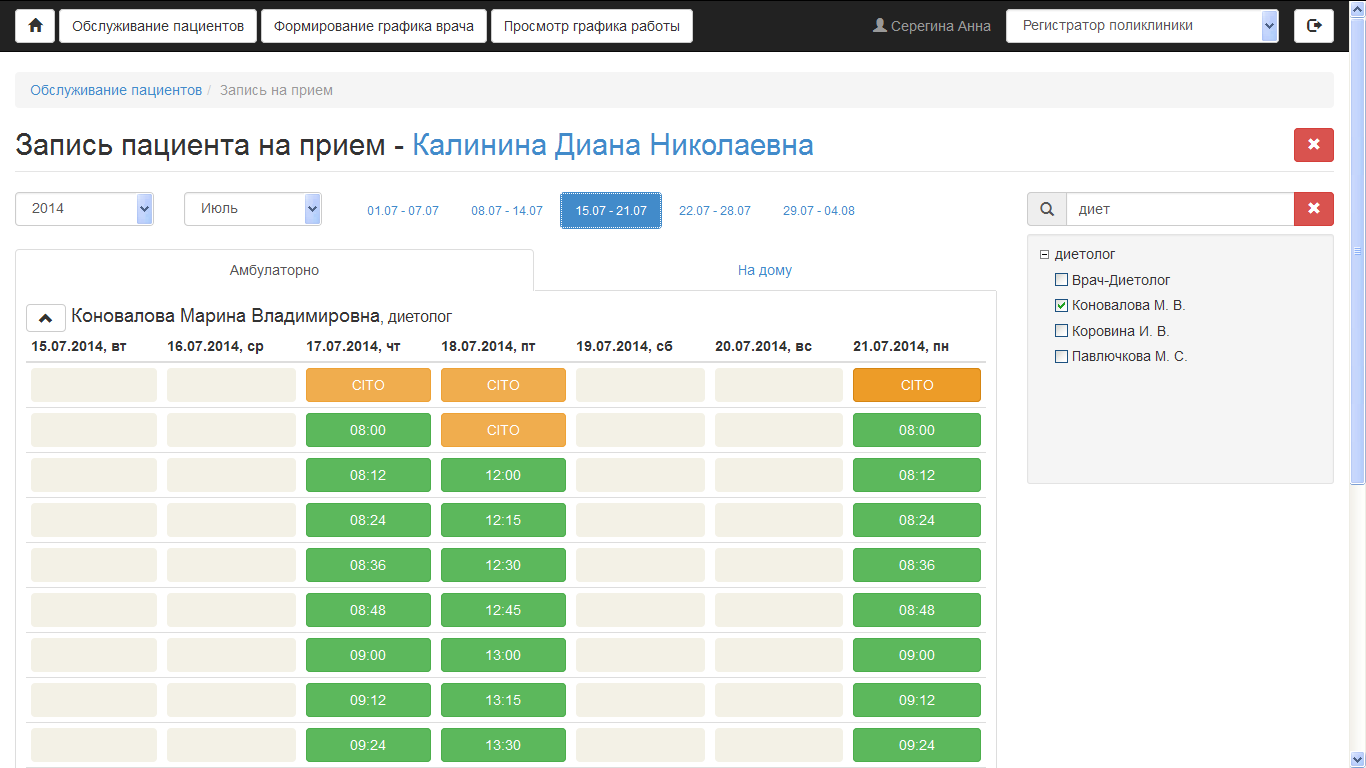
\includegraphics[width = 1\textwidth ,keepaspectratio]{pol_zapttbl}
  \caption{Запись пациента на прием}
  \label{img_pol_zapttbl}
 \end{figure}
 
 \item В случае наличия свободных талонов, щелкнуть по нему левой кнопкой мыши. Для перехода к следующей неделе, нужно выбрать соответствующий интеврал дат в верхней части страницы, под фамилией пациента.
 \item В появившемся всплывающем окне, нажать кнопку \btn{Ok}, подтверждающую запись пациента на прием. Выбранный интервал будет окрашен в красный цвет.
 \item Если пациент записан на прием успешно, то в поле \dm{ФИО} выбранного интервала появятся данные пациента. В секции 9 для этого пациента на вкладке \dm{Предварительная запись} так же добавится новая строка о предварительной записи к выбранному врачу. На экране появится окно просмотра печатной формы направления. Для печати направления нужно нажать кнопку \btn{Печатать}, для сохранения направления в файл – кнопку \btn{Сохранить}. Если печать направления не требуется, то следует нажать кнопку \btn{Закрыть}.
\end{enumerate}
  
В \tmis~реализована возможность экстренной записи и записи сверх нормы на выбранную дату. Для записи экстренного пациента, нужно выбрать в расписании талон оранжевого цвета с надписью <<CITO>>, расположенную в верхней части расписания врача. Для записи пациентов сверх нормы нужно выбрать в расписании талон серого цвета с надписью <<Сверх плана>>, расположенную внизу списка талонов на выбранный день. Количество экстренных пациентов и пациентов, записанных сверх плана, которые могут быть записаны к данному врачу на текущий день настраивается при создании расписания работы врача. 

Для отмены предварительной записи нужно щелкнуть по соответствующему талону красного цвета на странице записи пациентов на прием (Рисунок \ref{img_pol_zapttbl}) и в появившемся всплывающем окне <<Отменить запись на прием?>> нажать кнопку \btn{Ok}. Запись пациента на прием будет отменена, а талон осободится.

\subsection{Вызов врача на дом} \label{pol_home}

Принцип регистрации вызовов врача на дом в \tmis~аналогичен предварительной записи на прием. При регистрации вызова врача на дом следует перейти на вкладку \dm{На дому} в окне \dm{Запись пациента на прием} и выбрать интервал для записи на этой вкладке. Остальные действия аналогичны действиям при записи на амбулаторный прием.

\subsection {Регистрация обращений} \label{pol_obr}

Каждый раз при обращении пациента в ЛПУ за амбулаторной или поликлинической помощью, в картотеке пациентов для него регистрируется новое обращение. Обращение содержит цель, установленные диагнозы пациента, результаты осмотров и обследований, информацию о назначенных мероприятиях и их выполнении, результат обращения. На основании обращения можно распечатать <<Талон амбулаторного пациента>> (Ф. 025\slash У-12).

Для регистрации обращения на основе предварительной записи следует найти пациента в БД (см. п. \ref{cl_find}) и щелкнуть по нему левой кнопкой мыши. В появившемся всплывающем окне (Рисунок \ref{img_cl_contrwin}) нужно нажать кнопку 
\includegraphics[scale=0.6]{addg}, справа от соответствующей записи на вкладке \dm{Предварительная запись}. Будет открыта страница \dm{Создание обращения}.

Дле регистрации обращения без предварительной записи во всплывающем окне (Рисунок \ref{img_cl_contrwin}) нужно нажать кнопку \btn{Создать обращение} или кнопку 
\includegraphics[scale=0.6]{addb}. Если у пациента имеются предварительные записи к другим специалистам, то появится предупреждение во всплывающем окне <<У пациента есть предварительные записи>>. Для продолжения создания обращения следует нажать кнопку \btn{Все равно продолжить}, для отказа от создания обращения без предварительной записи нужно нажать кнопку \btn{Отмена}. В случае выбора продолжения создания обращения, будет открыта страница \dm{Создание обращения}. Кнопка \btn{Создать обращение} доступна так же из регистрационной карточки пациента.

На странице создания обращения, прежде всего, необходимо проверить, что обращение создано для нужного пациента, сверив его данные в правой верхней части окна. После этого нужно заполнить пустые и изменить неверно заполненные поля в блоке \dm{Основная информация}. Часть полей может быть заполнена на основе данных предварительной записи (если обращение создавалось на основе нее) или значениями по умолчанию.

\begin{vnim}
 Поля Дата выполнения и Время выполнения на данном этапе заполнять не нужно!
\end{vnim}

Все поля, кроме полей \dm{Дата выполнения} и \dm{Время выполнения} являются обязательными для заполнения.
\begin{itemize}
 \item \dm{Тип обращения} выбирается из списка значение <<Поликлиника>>.
 \item \dm{Источник финансирования} – канал оплаты обращения, выбирается из списка.
 \item \dm{Договор} – номер договора об оплате выбирается из списка. Состав списка зависит от выбранного источника финансирования.
 \item \dm{Тип события} – выбирается из списка. Состав списка изменяется в зависимости от выбранного типа обращения и источника финансирования.
 \item \dm{Лечащий врач} – врач, к которому направляется пациент в поликлинике.
 \item \dm{Подразделение} – отделение поликлиники, куда направляется пациент.
 \item \dm{Дата начала} – по умолчанию устанавливается дата предварительной записи либо текущая дата. При необходимости дату можно изменить.
 \item \dm{Время начала} – по умолчанию устанавливается время предварительной записи либо текущее время. При необходимости время можно изменить.
 \item \dm{Дата выполнения} – дата завершения обслуживания по данному обращению. Должна заполняться врачом.
 \item \dm{Время выполнения} – время закрытия обращения. Должно заполняться врачом.
\end{itemize}

После того как все поля заполнены верно, нужно нажать кнопку \btn{Создать} в правом нижнем углу страницы. Будет осуществлен переход к следующему этапу оформления обращения. Как правило, работа регистратуры ограничивается первым этапом. Последующее заполнение обращения выполняется врачом.

Если была предпринята попытка создания обращения не для того пациента или создание обращения вообще не требуется, следует нажать кнопку \btn{Отменить}. Обращение создано не будет.